%%%%%%%%%%%%%%%%%%%%%%%%%%%%%%%%%%%%%%%%%%%%%%%%%%%%%%%%%%%%%%%%%%%%%%%%%%%%%%%%
\documentclass[presentation]{beamer}\mode<presentation>{\usetheme{sapere}}
%
\usepackage[english]{babel}
\usepackage[utf8]{inputenc}
\usepackage{beamersapere}
\usepackage{amssymb}
%\usepackage{makeidx}  % allows for indexgeneration
\usepackage{graphicx}
\usepackage{subfigure}
\usepackage{subcaption}
\usepackage{wrapfig}
\usepackage{amsmath,amssymb,stmaryrd,mathtools,alltt}
\usepackage{inputenc}
\usepackage{fontenc}
\usepackage{url}
\usepackage{multimedia,pgf}
\usepackage{geometry}
\usepackage{listings}
\usepackage{framed}
\usepackage{tabularx}
\usepackage[active]{srcltx}
% \usepackage{tikz}
\usepackage{array}
\usepackage{cleveref}

\newcommand{\plocation}{\texttt{\#location}}
\newcommand{\hasany}{\texttt{has}}
\newcommand{\hasnot}{\texttt{hasnot}}
\newcommand{\hasone}{\texttt{=}}
\newcommand{\assign}{\texttt{:=}}
\newcommand{\extends}[1]{\texttt{extends~#1}}
\newcommand{\clones}[1]{\texttt{clones~#1}}
\newcommand{\annvar}[2]{\{#1:#2\}}

\renewcommand{\ttdefault}{txtt}
\newcommand{\ssum}{+}
\newcommand{\strn}[1]{--#1-->}
\newcommand{\strninf}{--->}
\newcommand{\spatt}[2]{#1:[#2]}
\newcommand{\spattid}[1]{#1}
\newcommand{\sseq}{;}
\newcommand{\sclones}[1]{clones #1}
\newcommand{\sextends}[1]{extends #1}
\newcommand{\shasall}{=*}
\newcommand{\shasany}{~\texttt{has}~}
\newcommand{\shasnot}{~\texttt{has-not}~}
\newcommand{\shasone}{\texttt{=}}
\newcommand{\sis}{\texttt{=}}
\newcommand{\svar}[1]{#1}
\newcommand{\sid}[2]{?(#1[#2])}
\newcommand{\svardesc}[1]{#1}
\newcommand{\sannvar}[2]{?\{#1:#2\}}
\newcommand{\slist}[1]{(#1)}
\newcommand{\sdesc}[1]{[#1]}
\newcommand{\sliteral}[1]{"#1"}
\newcommand{\sprop}[1]{\sliteral{#1}}
\newcommand{\erase}[1]{|#1|}
\newcommand{\pattern}[2]{#1[#2]}
\newcommand{\shfiring}[1]{#1^\rightsquigarrow}

\newcommand{\tap}[1]{#1}
\newcommand{\local}{\texttt{local}}
\newcommand{\neighborhood}{\texttt{neighborhood}}
\newcommand{\globalc}{\texttt{global}}
\newcommand{\lsa}[1]{\langle #1\rangle}
\newcommand{\alchemist}[0]{{\tap{\textsc{Alchemist }}}}
\newcommand{\rem}[1]{+#1}


% \setbeamertemplate{background canvas}{\includegraphics[width=\paperwidth,height=\paperheight]{imgs/background.jpg}}
%%%% Title
\title[Engineering Computational Ecosystems]{Engineering Complex Computational Ecosystems}

\author[Danilo Pianini]
{\textbf{Danilo Pianini} \\ Supervisor: prof. Mirko Viroli \\ Tutor: prof. Antonio Natali
\\
\footnotesize danilo.pianini@unibo.it}

\institute[UniBo]
{\textsc{Alma Mater Studiorum}---Universit\`a di Bologna \\
}


\AtBeginSection[]
{
  \begin{frame}<beamer>
    \frametitle{Outline}
    \tableofcontents[currentsection]
  \end{frame}
}

\date[\today{} / Bologna]{Final Exam of the ET-IT Program XXVII Cycle \\ Dipartimento di Ingegneria dell'Energia Elettrica e dell'Informazione ``Guglielmo Marconi''}


\pgfdeclareimage[height=0.625cm]{university-logo}{imgs/logo}
\logo{\pgfuseimage{university-logo}}


\begin{document}


%===============================================================================
\frame[label=coverpage]{\titlepage}
%===============================================================================

\section*{Outline}
\subsection*{Accepting the limitations of birthform betrays lack of imagination}
%===============================================================================
\frame{\tableofcontents}


\section{Set the stage}

\subsection{Towards a pervasive world}

\begin{frame}{Pervasive Devices}
  \centering
  \scriptsize
  Image courtesy of Alois Ferscha (Pervasive Computing Group, Johannes Kepler Universität Linz)
  \begin{figure}
    \includegraphics[width=0.85\textwidth]{imgs/devices} 
  \end{figure}
\end{frame}

\begin{frame}{Progress look pretty normal when you look back...}
  \centering
  \scriptsize
   Image from Tim Urban's ``Wait but why'' blog (http://waitbutwhy.com/)
  \begin{figure}
    \includegraphics[
%      width=\textwidth,
      height=0.8\textheight
      ]{imgs/Edge} 
  \end{figure}
\end{frame}

\begin{frame}{...but fasten your belt anyway, please}
  \centering
  \scriptsize
  Image from Tim Urban's ``Wait but why'' blog (http://waitbutwhy.com/)
  \begin{figure}
    \includegraphics[
%      width=\textwidth,
      height=0.8\textheight
      ]{imgs/Edge1} 
  \end{figure}
\end{frame}

\subsection{Engineering a pervasive world}

\begin{frame}{The hard part}
\begin{block}{Challenges}
\begin{itemize}
 \item Interaction can be P2P, centralised, or likely mixed
 \item Devices may or may not be mobile
 \item Desired behaviour may change greatly in response to changes in the local environment
 \item Evolution of deployed systems is generally unpredictable
\end{itemize}
\end{block}
\end{frame}

\begin{frame}{Issues for engineers}
   \begin{block}{Lack of design patterns}
      The closest thing are nature inspired patterns, that make the aggregate of devices expose some emergent behaviour in a robust, adaptive and distributed fashion \cite{ecosystems-jpcc7}. Nature is cool, but not always optimal.
   \end{block}
%    \begin{block}{Local-to-global issues}
%       Classic per-device programming does not provide the desired abstraction level, since system's goals happen at a global level. Interaction and protocols are mechanisms that we would like to hide.
%    \end{block}
% \end{frame}
% \begin{frame}{Issues for engineers}
   \begin{block}{Languages}
      Few languages explicitly target the aggregate of devices rather than the single one.
%       \begin{itemize}
%          \item MIT Proto \cite{proto} is probably the best example, it actually has an implementation and works both in simulators and real devices, but has a really complex underlying operational semantics \cite{spatialcomputing-sac11, proto-semantics-full}.
%          \item Field calculus \cite{VDB-FOCLASA-CIC2013} is a distilled version of Proto, with a clear and compact operational semantics, but no real world implementation.
%       \end{itemize}
   \end{block}
   \begin{block}{Verification}
%       \begin{itemize}
%          \item
Unpredictability widen the spectrum of possible evolutions, which make unit testing and model checking not feasible: simulation is often the only way to go
%       \end{itemize}
   \end{block}
\end{frame}

\begin{frame}{Contribution of this PhD}
\begin{block}{A toolchain for software ecosystems \cite{alchemist-jos2013}}
\begin{itemize}
 \item Meta-meta-model supporting very different approaches
 \item Built-in, SSA inspired, novel simulation engine
 \item Probabilistic and distributed model checking \cite{alchemist-multivesta}
\end{itemize}
\end{block}
\begin{block}{A language for aggregate programming \cite{protelis}}
\begin{itemize}
 \item Based on field calculus: formal and lightweight operational semantics
 \item The same code runs in simulator and real world devices
 \item Interoperability with Java (no need to reinvent the wheel)
\end{itemize}
\end{block}
\begin{block}{Self-organisation patterns and possible today's applications}
\begin{itemize}
   \item Crowd steering \cite{sapereecolaws-sac2012, serene-evacuation, hpcs2014, crowd-prediction}
   \item Resource discovery \cite{resource-discovery}
   \item Anticipative adaptation \cite{anticipativegradient-SASO12}
\end{itemize}
\end{block}
\end{frame}

\section{Alchemist: an integrated toolchain for complex ecosystems}
\begin{frame}{What is it}
\begin{block}{Idea}
\begin{itemize}
 \item A simulator was needed for the European project SAPERE \cite{sapere-procedia7}
 \item SAPERE adopts a chemical-like metaphor \cite{ker2014}
 \item Stochastic chemical simulators (SSA) are extremely efficient \cite{gibson2000, slepoy2008}
 \item Rather than relying on existing ABMs, very expressive but not as scalable as we desired, let's extend SSAs to be able to express what we want \cite{mass2011}
\end{itemize}
\end{block}
The simulator evolved beyond its original purposes to the point where it stands now.
\end{frame}

\subsection{Computational model}

\begin{frame}{Generalised chemistry}
\begin{block}{Pure chemistry vs. pervasive computing}
\begin{itemize}
 \item Single, static compartment versus multiple, possibly mobile, and interconnected nodes whose connection may depend on environmental and technological factors
 \item Molecules are described by concentration (an integer), devices may carry any kind of data item
 \item Reactions ``scheduling'' in nature follows a Poisson distribution whose rate equation depends on reagents' concentration \cite{gillespie1977}. Events in a pervasive computing scenario may be influenced by any of the environment components and follow any probability distribution (triggers, timers, and people walking are not Markovian)
 \item Devices live in an environment
\end{itemize}
\end{block}
Yes, it is a nicely big leap
\end{frame}

\begin{frame}{Close the gap: environment}
  \begin{figure}
    \includegraphics[
%       width=\textwidth,
      height=0.8\textheight
      ]{imgs/newmodel/model} 
  \end{figure}
\end{frame}

\begin{frame}{Close the gap: reactions}
  \begin{figure}
    \includegraphics[
      width=\textwidth,
%      height=0.8\textheight
      ]{imgs/reaction} 
  \end{figure}
\end{frame}

\begin{frame}{((Meta) Meta) Models}
\begin{block}{Meta levels explained}
\begin{itemize}
 \item The simulated instance of the system, or scenario, is the \textbf{model}
 \item The specific concentration type (e.g. integer, tuple, or even Java Object) along with specific actions and conditions that act upon such data type represents the meta-model (in the Alchemist jargon, ``incarnation'').
 \item The components of the Alchemist abstract computational model are the meta-meta model, which is common to all incarnations (and, in turn, to all scenarios).
\end{itemize}
\end{block}
\end{frame}

\subsection{Engine, architecture, tools}
\begin{frame}{Architecture}
  \begin{figure}
    \includegraphics[
      width=\textwidth,
%       height=0.8\textheight
      ]{imgs/architecture} 
  \end{figure}
\end{frame}

\begin{frame}{Engine}
   \begin{block}{}
      \begin{itemize}
       \item Full fledged Discrete Event Simulator derived from Gibson/Bruck SSA, extended with novel structures
       \item Supports dependency graph among reactions (this \textbf{really} boosts performance)
       \item Supports execution ``contexts'', pruning the dependency graph, strongly boosting the boost
      \end{itemize}
   \end{block}
  \begin{figure}
    \includegraphics[
%       width=\textwidth,
      height=0.5\textheight
      ]{imgs/jos-perf} 
  \end{figure}
\end{frame}

\begin{frame}{Handle with care}
\begin{block}{When is Alchemist worth it?}
\begin{itemize}
 \item An incarnation exposing the desired level of abstraction is already available: faster and closer to the model than a generic ABM
 \item There is a long-term investment on Alchemist, and a new incarnation is developed: performance pay back the investment
\end{itemize}
\end{block}
\begin{block}{Incarnations available}
\begin{itemize}
 \item \textbf{Pure chemistry} -- Little more than an incubation test, deprecated
 \item \textbf{SAPERE} -- Mature incarnation, simulates a network of programmable tuple spaces. Programs are chemical-like tuple re-writing rules 
 \item \textbf{Protelis} -- Supports the execution of Protelis programs on networks of simulated devices. Usable, but under heavy development.
 \item \textbf{Biochemistry} -- Sketched, will replace chemistry, exposing much better support for biological oriented applications (back to the fold)
\end{itemize}
\end{block}
\end{frame}

\section{Aggregate programming}

\subsection{Paradigm shift: programming space/time}
\begin{frame}{Classic approach}
\begin{block}{Local to global}
  \begin{itemize}
    \item Complex global behaviour
    \item Simple local behaviour
    \item The whole is more than the sum of the parts
    \item Interaction is key
  \end{itemize}
\end{block}
\begin{block}{Nature inspiration}
   Several systems use nature as inspiration:
  \begin{itemize}
    \item physical particles \cite{mamei2009acm}
    \item chemical reactions \cite{sapere-procedia7}
    \item ants, termites and other social insects \cite{swarmlinda}
    \item Very brief list! There are many more.
  \end{itemize}
\end{block}
\end{frame}

\begin{frame}{Nice properties and hard challenges}
  \begin{block}{The beauty}
    \begin{itemize}
      \item High resilience and fault tolerance
      \item Self adaptation
      \item Openness
      \item Self healing
    \end{itemize}
  \end{block}
  \begin{block}{The beast}
    Local to global is hard to engineer
    \begin{itemize}
      \item The desired functionality happens at the aggregate level
      \item It is very difficult to design the local behaviour in such a way that the interaction of many of them produces the desired global behaviour
      \item Many attempts, but no good engineering processes to safely design such systems
      \item Often, development becomes a try-and-simulate loop
    \end{itemize}
  \end{block}
\end{frame}

\begin{frame}{Collective to local}
  \begin{block}{Desiderata}
    \begin{itemize}
      \item We want to achieve a collective behaviour
      \item We want to move our focus and abstractions towards the \emph{the whole network}, rather than focussing on the single devices that compose it and their interaction
      \item We want to support space-time abstractions
    \end{itemize}
  \end{block}
  \begin{block}{Possible solution}
    \begin{itemize}
      \item Create a language that allows to express collective properties
      \item Create a runtime that can run such programs
      \begin{itemize}
         \item Possibly, also create a tool to test programs prior to deployment
      \end{itemize}
    \end{itemize}
  \end{block}
\end{frame}

% \subsection{From Proto to Field Calculus}
\begin{frame}[fragile]{Real languages}
\begin{block}{Aggregate programming languages}
   \begin{itemize}
    \item Several attempts to bring existing languages to the aggregate perspective, we tried with Linda \cite{VPB-COORD2012}
   \end{itemize}
\end{block}
  \begin{block} {MIT Proto \cite{proto} is the most known and successful}
   \begin{itemize}
    \item Developed at MIT and maintained at BBN Technologies
    \item Functional language, LISP-like syntax (I know you hate it too)
    \item \emph{All devices run the same program}
    \item Computation happens in rounds:
    \begin{itemize}
      \item Every device sleeps for some time
      \item Processes the messages received from the neighbours
      \item Executes its program
      \item Sends all the neighbours its result
    \end{itemize}
    \item Complex operational semantics
   \end{itemize}
  \end{block}
\end{frame}

\begin{frame}[fragile]{Field Calculus}
  \begin{block} {A ``distillate'' of Proto}
   \begin{itemize}
    \item Provides a lightweight operational semantics \cite{VDB-FOCLASA-CIC2013}
    \item ((((LISP-like syntax))))
    \item Still a functional language
    \item Simple enough to formally prove properties, powerful enough to be universal (proved!)
    \item Theoretical object, no runtime nor simulation tool provided
   \end{itemize}
  \end{block}
  \begin{block} {Key mechanism: alignment}
   \begin{itemize}
    \item At the end of each cycle, send to your neighbours your annotated AST
    \item At the beginning of each cycle, each device can inspect what was happening in its surroundings
    \item If two devices took different branches of a \texttt{if}, they are no longer aligned until such branch returns
   \end{itemize}
  \end{block}
\end{frame}

\subsection{Protelis: practical aggregate programming}

\begin{frame}{Protelis}
  \begin{block} {}
   \begin{itemize}
    \item Functional language
    \item Same operational semantics of the field calculus 
    \item Java-like syntax with infix operators
    \item Java interoperability: static methods imports and calls, method invocation with dynamic binding
    \item \textbf{Higher order functions (functions as arguments, closures, lambdas)}
    \item \textbf{Dynamic code}
    \item Eclipse plugin
    \item Integrated with Alchemist
    \item Stand-alone framework for real devices
    \item Write once, run everywhere --- evolved :)
   \end{itemize}
  \end{block}
\end{frame}

\begin{frame}{Alignment with HOF}
  \begin{block} {How to deal with alignment?}
   \begin{itemize}
    \item     Without HOF, all the devices are forced to run the same code: the only branching point is \texttt{if}.
    \item With HOF, and in particular with support for dynamic code, instead:
    \scriptsize
    \begin{enumerate}
      \item The same function can be defined in multiple points
      \item Different functions may have the same name (dynamic injection)
      \item The same function can be invoked in multiple points
      \item The same code path may invoke a different function
    \end{enumerate}
   \end{itemize}
  \end{block}
  \begin{block} {Alignment}
    Alignment had been improved to consider HOF support.
   Two functions align only if:
    \begin{itemize}
      \item They have the same name and body
      \item They were defined in the exact same point in code
      \item They are invoked in the exact same point in code
    \end{itemize}
  \end{block}
\end{frame}

\begin{frame}[fragile]{LISP-like to Java-like syntax}
    \scriptsize
    \begin{lstlisting}[mathescape,morekeywords={rep,mux,sense,inf,def,min,hood,nbr,nbr,range,else,if,Infinity},numbers=left,basicstyle=\ttfamily]
(def distance-to (source)
  (rep d infinity (mux source 0 (min-hood (+ (nbr d) (nbr-range))))))
distance-to(event)
    \end{lstlisting}
    ~ \\ ~ \\ ~ \\
    \scriptsize
    \begin{lstlisting}[mathescape,morekeywords={rep,mux,sense,inf,def,minHood,nbr,nbr,nbrRange,else,if,Infinity},numbers=left,basicstyle=\ttfamily]
def distanceTo(source) {
  rep (d <- Infinity) {
    mux (source) {
      0
    } else {
      minHood(nbr(d) + nbrRange)
    }
}
distanceTo(event)
    \end{lstlisting}
\end{frame}

\begin{frame}[fragile]{Example with HOF}
    \tiny
    \begin{lstlisting}[mathescape,morekeywords={rep,mux,sense,inf,def,min,hood,nbr,nbr,range,else,if,Infinity},numbers=left,basicstyle=\ttfamily]
def gBB(source, initial, metric, accumulate) {
   rep(distanceValue <- [Infinity, initial]) {
      mux(source) {
         [0, initial]
      } else {
         let ndv = nbr(distanceValue);
         minHood([ndv.get(0) + metric.apply(), accumulate.apply(ndv.get(1))])
      }
   }.get(1)
}

def distanceCompetition(d, lead, uid, grain, metric) {
   mux(d > grain * 1.5) { uid } else {
      let gsize = grain * 0.5;
      mux (d >= gsize) { Infinity } else {
         minHood(mux(nbr(d) + metric.apply() >= gsize) { Infinity } else { nbr(lead) })
      }
   }
}

def breakUsingUIDs(uid, grain, metric) {
   uid == rep(lead <- uid) {
      distanceCompetition(
         gBB(uid == lead, 0, metric, (v) -> {v + metric.apply()}), lead, uid, grain, metric)
   }
}

breakUsingUIDs(grain, metric)
    \end{lstlisting}
\end{frame}



\section{Future technology applied today}

\begin{frame}{Applications for densely populated environments}
  \begin{block}{Crowd steering and evacuation}
    \begin{itemize}
     \item Provide guidance to prevent dangerous situations, e.g.:
      \begin{itemize}
      \item In case of emergency, dynamically balance the crowds to minimize the evacuation time
      \item Avoid crowded paths when providing directions
      \item Prevent dangerous crowd formation
      \item Alert users joining a dangerous cluster
      \end{itemize}
    \end{itemize}
  \end{block}
  \begin{block}{Other services}
    \begin{itemize}
     \item Local communication
     \item Context sensitive applications
     \item Local services and advertisement
    \end{itemize}
  \end{block}
\end{frame}

\begin{frame}{Crowd-sensitive user steering}
{\footnotesize Steering against GPS traces taken at Vienna City Marathon 2013}
\begin{center}
  \movie[width=12cm,height=6.6cm,showcontrols=true,poster]{}{video/wien.webm}
\end{center}
\end{frame}

\begin{frame}{Context sensitive user steering}
{\footnotesize Generalisation of the former, ran in London}
\begin{center}
  \movie[width=12cm,height=6.6cm,showcontrols=true,poster]{}{video/london.webm}
\end{center}
\end{frame}

\begin{frame}{Mobile code}
  \centering
  \begin{figure}
    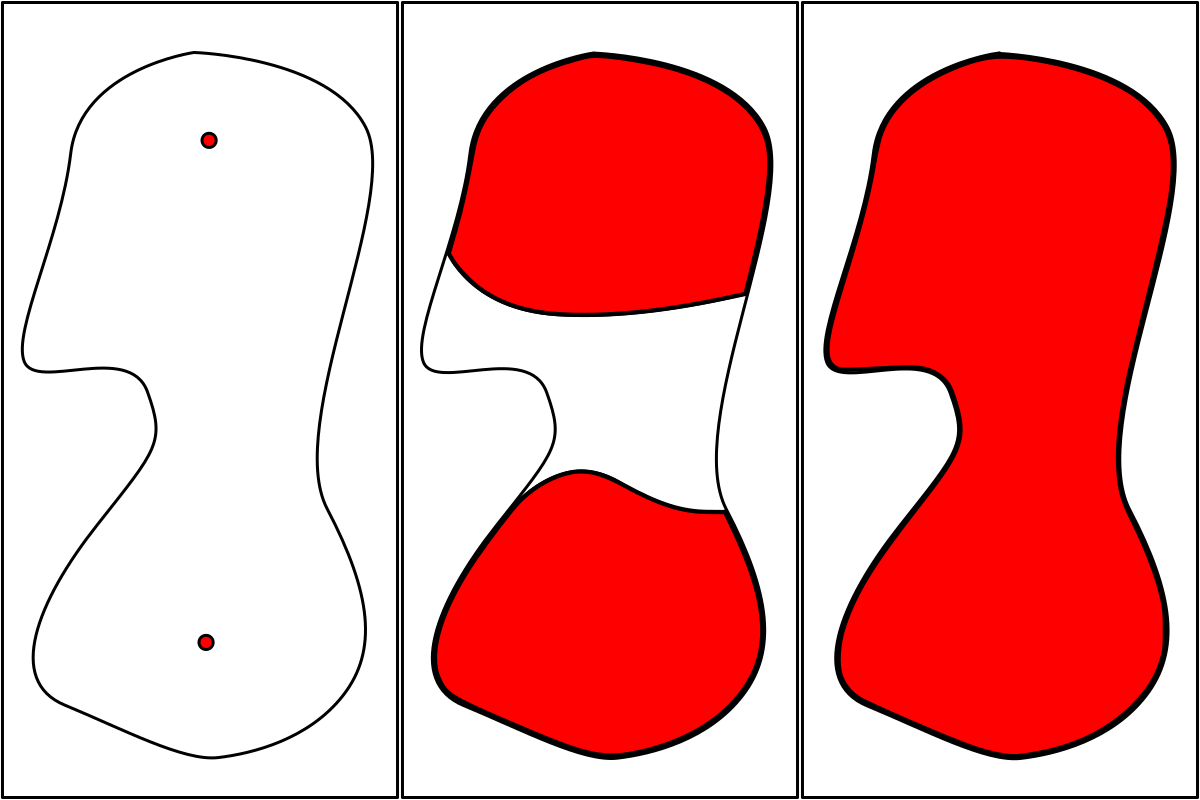
\includegraphics[width=0.7\textwidth]{imgs/inject} 
  \end{figure}
\end{frame}

\begin{frame}[fragile]{Upgradable mobile code}
\begin{center}
  \movie[width=12cm,height=7cm,showcontrols=true,poster]{}{video/inject.ogv}
\end{center}
\end{frame}

\begin{frame}{Upgradable mobile code}
  \centering
  \begin{figure}
    \includegraphics[width=0.7\textwidth]{imgs/upgrade} 
  \end{figure}
\end{frame}

\begin{frame}[fragile]{Upgradable mobile code}
\begin{center}
  \movie[width=12cm,height=7cm,showcontrols=true,poster]{}{video/upgradable.ogv}
\end{center}
\end{frame}

\begin{frame}{Overlapping services}
  \centering
  \begin{figure}
    \includegraphics[width=0.8\textwidth]{imgs/restaurants2} 
  \end{figure}
\end{frame}

\begin{frame}[fragile]{Overlapping services}
\begin{center}
  \movie[width=12cm,height=7cm,showcontrols=true,poster]{}{video/overlapping.ogv}
\end{center}
\end{frame}



\section{Conclusion and future work}

\subsection*{Results}
\begin{frame}{Results}
\begin{block}{A toolchain for software ecosystems}
\begin{itemize}
 \item Novel, chemical inspired architecture, developed from scratch
 \item Flexible still retaining high performace
\end{itemize}
\end{block}
\begin{block}{A language for aggregate programming \cite{protelis}}
\begin{itemize}
 \item Based on Field Calculus, lightweight semantics
 \item Support for higher order functions, closures, code injection
 \item Integrated development: write your program, run both in Alchemist and real devices
\end{itemize}
\end{block}
\begin{block}{Self-organisation patterns and possible today's applications}
\begin{itemize}
  \item Novel self-organisation patterns
  \item Application of existing and novel patterns to crowd steering, WSN and other high- density scenarios
\end{itemize}
\end{block}
\end{frame}

\subsection*{Future works}
\begin{frame}{Future development}
\begin{block}{A toolchain for software ecosystems}
\begin{itemize}
 \item Stabilise development, strenghten existing features
 \item Include interactivity
 \item Rethink the distributed approximate model checker
 \item Complete biochemistry incarnation
\end{itemize}
\end{block}
\begin{block}{A language for aggregate programming}
\begin{itemize}
 \item Are we about to create distributed processes?
 \item Protelis could be a nice language for distributed service scheduling
 \item Enable better modularity
 \item Strong type checking
\end{itemize}
\end{block}
\begin{block}{Self-organisation patterns and possible today's applications}
\begin{itemize}
  \item Create a rich library of reusable building blocks for self-* application
\end{itemize}
\end{block}
\end{frame}


%===============================================================================
\section*{\refname}
%===============================================================================
\begin{frame}[allowframebreaks]
%\begin{frame}[t,allowframebreaks]
  \frametitle{\refname}
  \scriptsize
  \bibliographystyle{alpha}
  \bibliography{bibliography}
\end{frame}
\section*{\refname}
%===============================================================================

\againframe{coverpage}

\section*{Alchemist: director's cut}

\begin{frame}{Model to model}
\begin{block}{Generic procedure}
\begin{enumerate}
 \item Map your meta model onto Alchemist's meta-meta model entities
 \item Optionally, write a Domain Specific Language (DSL) which generates an Alchemist-XML compatible file from your domain-specific entities
 \item Write whichever model you want to test and simulate
 \item Simulate it using Alchemist
\end{enumerate}
\end{block}
\end{frame}

\begin{frame}{}
% \frametitle{Smart data structures ensure bleeding edge performances}
\begin{figure}[H]
  \begin{center}
    \includegraphics[width=0.485\textwidth]{imgs/extipq.pdf}
    \hspace{30pt}
    \includegraphics[width=0.39\textwidth]{imgs/dependencygraph.pdf}
    \label{img:datastruct}
  \end{center}
\end{figure}
\begin{block}{Next Reaction efficient structures made dynamic}
\begin{itemize}
 \item Dynamic Indexed Priority Queue
\begin{itemize}
 \item Allow to access the next reaction to execute in O(1) time
 \item Worst case update in $\log_2{(N)}$ (average case a lot better)
 \item Extended to ensure balancing with insertion and removal
\end{itemize}
 \item Dynamic Dependency Graph
\begin{itemize}
 \item Allows to smartly update only a subset of all the reaction
 \item Extended with the concept of input and output context
\end{itemize}
\end{itemize}
\end{block}
\end{frame}

\begin{frame}{Real world maps and GPS traces}
  \begin{figure}
    \includegraphics[width=\textwidth]{imgs/vienna}
    \caption{A snapshot of the whole city of Vienna as simulated in Alchemist. This snapshot is taken while simulating the city at 10am during the annual marathon, each black point corresponds to a GPS trace.}
    \label{img:vienna}
  \end{figure}
\end{frame}

\begin{frame}{Approximate Stochastic Model Checker}
\begin{block}{Problem}
 \begin{itemize}
  \item Model checking is not feasible with such complexity, but Monte Carlo sampling is
  \item How many simulations should you run to in order to get the mean value of some property, along with its confidence and approximation?
 \end{itemize}
\end{block}
\begin{block}{Alchemist + MultiVeStA}
 \begin{itemize}
  \item Alchemist has been chained with MultiVeStA
  \item A properties can be written in MultiQuaTeX
  \item MultiVeStA runs the number of experiments required using the chained Alchemist engine
  \item Big plus: MultiVeStA supports distributed execution
 \end{itemize}
\end{block}
\end{frame}



\section*{Aggregate programming: director's cut}

\begin{frame}[fragile]{Example}
    \scriptsize
    \begin{lstlisting}[mathescape,morekeywords={rep,mux,sense,inf,def,min,hood,nbr,nbr,range,else,if,Infinity},numbers=left,basicstyle=\ttfamily]
(def distance-to (source)
  (rep d infinity (mux source 0 (min-hood (+ (nbr d) (nbr-range))))))
distance-to(event)
    \end{lstlisting}
  \centering
  \begin{figure}
    \includegraphics[width=0.99\textwidth]{imgs/grad} 
  \end{figure}
\end{frame}

\begin{frame}{We want to do more}
  \begin{block} {Dynamic and mobile code with higher order functions}
   \begin{itemize}
    \item Functions can be arguments and can be returned 
    \item Closures
    \item Anonymous functions
    \item Dynamic code
   \end{itemize}
  \end{block}
  \begin{block} {Sugar and utilities}
   \begin{itemize}
    \item Java interoperability
    \item C family like syntax
   \end{itemize}
  \end{block}
\end{frame}

\begin{frame}[fragile]{Upgradable mobile code}
  \scriptsize
    \begin{lstlisting}[mathescape,morekeywords={import,as,def,if,rep,mux,sense,inf,let,eval,max,def,min,hood,nbr,nbr,range,else,Infinity},numbers=left,basicstyle=\ttfamily]
def upgrade (injection) {
  rep (versioned <- [0, "\"no program installed.\""]) {
    max-hood (nbr (
      if (injection.get(0)) {
        if(versioned < injection) { 
          injection
        } else {
          versioned
        }
      } else {
        versioned
      }
    ))
  }
}
let prog = upgrade([version, code]);
let code = prog.get(1);
eval(code);
    \end{lstlisting}
\end{frame}

\begin{frame}[fragile]{Overlapping services}
  \scriptsize
    \begin{lstlisting}[mathescape,morekeywords={import,as,def,if,rep,mux,sense,inf,let,eval,max,def,min,hood,nbr,nbr,range,else,Infinity},numbers=left,basicstyle=\ttfamily]
def map(f, t){
  if (t.isEmpty()) {
    t
  } else {
    [f.apply(t.get(0))].mergeAfter(map(f, t.subTupleEnd(1)))
  }
}
def distanceTo(source) {
  rep (d <- Infinity) {
    mux (source) { 0 } else { min-hood (nbr(d) + nbr-range) }
  }
}
def inRange(source, r) { distanceTo(source) < r }
/* actual program */
let services = [service0, service1, service2];
map((s) -> {
  if(inRange(s)) {
    eval(s)
  } else {
    "out of range"
  }
}, services);
\end{lstlisting}
\end{frame}

\begin{frame}[fragile]{Simpler semantics}
  \begin{columns}
    \begin{column}{6cm}
      \centering
      Proto \\
      \begin{framed}
        \includegraphics[width=0.31\columnwidth]{imgs/protosem1} 
        \includegraphics[width=0.35\columnwidth]{imgs/protosem2} \\
        \includegraphics[width=0.30\columnwidth]{imgs/protosem10} 
        \includegraphics[width=0.37\columnwidth]{imgs/protosem11}
        \includegraphics[width=0.30\columnwidth]{imgs/protosem12} \\
        \includegraphics[width=0.40\columnwidth]{imgs/protosem14} \\
        \includegraphics[width=0.39\columnwidth]{imgs/protosem13} 
        \includegraphics[width=0.59\columnwidth]{imgs/protosem16} \\
        \includegraphics[width=0.49\columnwidth]{imgs/protosem15} 
        \includegraphics[width=0.49\columnwidth]{imgs/protosem17} 
      \end{framed}
    \end{column}
    \begin{column}{6cm}
      \centering
      Field calculus \\
      \begin{framed}
        \includegraphics[width=1.015\columnwidth]{imgs/fcsem}
      \end{framed}
   \end{column}
  \end{columns}
\end{frame}

\begin{frame}{Key mechanism: Alignment}
  \begin{block} {Abstract syntax trees in Field Calculus}
   \begin{itemize}
    \item Representation of the abstract syntactic structure of a program
    \item The computation modifies every node of the tree, associating the corresponding value to it
    \item At the end of the round, it is sent to every neighbour
    \item During the round, each device can read the data every other node had at the same point in the code, and use it
    \item If some neighbour has not any data associated with the code path, it means that it has chosen a different branch
    \item Such node would be \textbf{not aligned}, and not considered for subsequent computation
   \end{itemize}
  \end{block}
\end{frame}

\begin{frame}[fragile]{Example}
    \begin{lstlisting}[mathescape,morekeywords={rep,mux,sense,inf,def,min,hood,nbr,nbr,range,else,if,Infinity},numbers=left,basicstyle=\ttfamily]
(if (> x 0) (x + 1) (x - 1))
    \end{lstlisting}
  \centering
  \begin{figure}
    \includegraphics[width=0.9\textwidth]{imgs/ast} 
  \end{figure}
\end{frame}

\begin{frame}[fragile]{Example}
  \centering
  \begin{figure}
    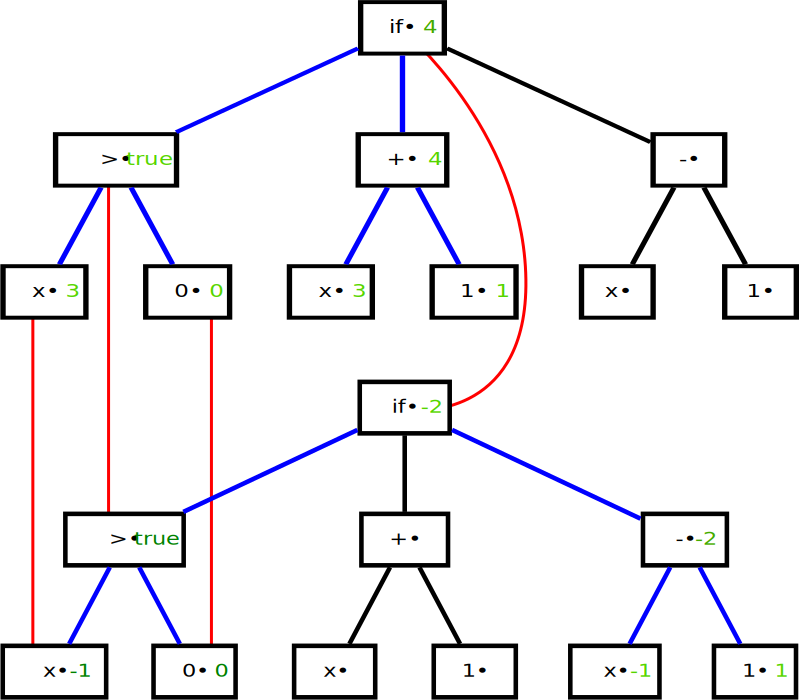
\includegraphics[width=0.6\textwidth]{imgs/trees} 
  \end{figure}
\end{frame}

\begin{frame}{Conclusion}
  \begin{block} {Aggregate programming}
   \begin{itemize}
    \item Focus on the whole network
    \item Think in space and time
    \item Much less focus on communication protocols
    \item Paradigm shift: requires training!
   \end{itemize}
  \end{block}
  \begin{block} {Protelis}
   \begin{itemize}
    \item Solid foundations (field calculus)
    \item Support for higher order functions
    \item Interoperability with Java
    \item Friendly syntax
    \item Simulation framework
   \end{itemize}
  \end{block}
\end{frame}

\begin{frame}{Future work}
  \begin{block} {Language side}
   \begin{itemize}
    \item Sugar, sugar, sugar
    \item Namespacing (done by now, if no disasters happened just before this dissertation)
    \item Libraries
   \end{itemize}
  \end{block}
  \begin{block} {Tools side}
   \begin{itemize}
    \item Distributed middleware
    \item Better simulator UI
    \item Better batch executor and logging service
    \item Tons of documentation
   \end{itemize}
  \end{block}
\end{frame}

\section*{Self-org patterns: director's cut}

\begin{frame}{Why crowds}
  \begin{block}{}
    We are preparing for a world that does not exist yet.
  \end{block}
  \begin{block} {Why we often focus on crowds}
   \begin{itemize}
    \item Smallest and most diffused devices in today's world are normally accessories or wearables
    \item The higher density of people, the higher density of devices
    \item Challenging issues to tackle, including low reliability of Internet connection
   \end{itemize}
  \end{block}
  \begin{block}{}
    Crowds of people are real world scenarios available today that closely resemble our future pervasive world.
  \end{block}
\end{frame}

\begin{frame}{Today's infrastructure}
  \centering
  \scriptsize
  \begin{figure}
    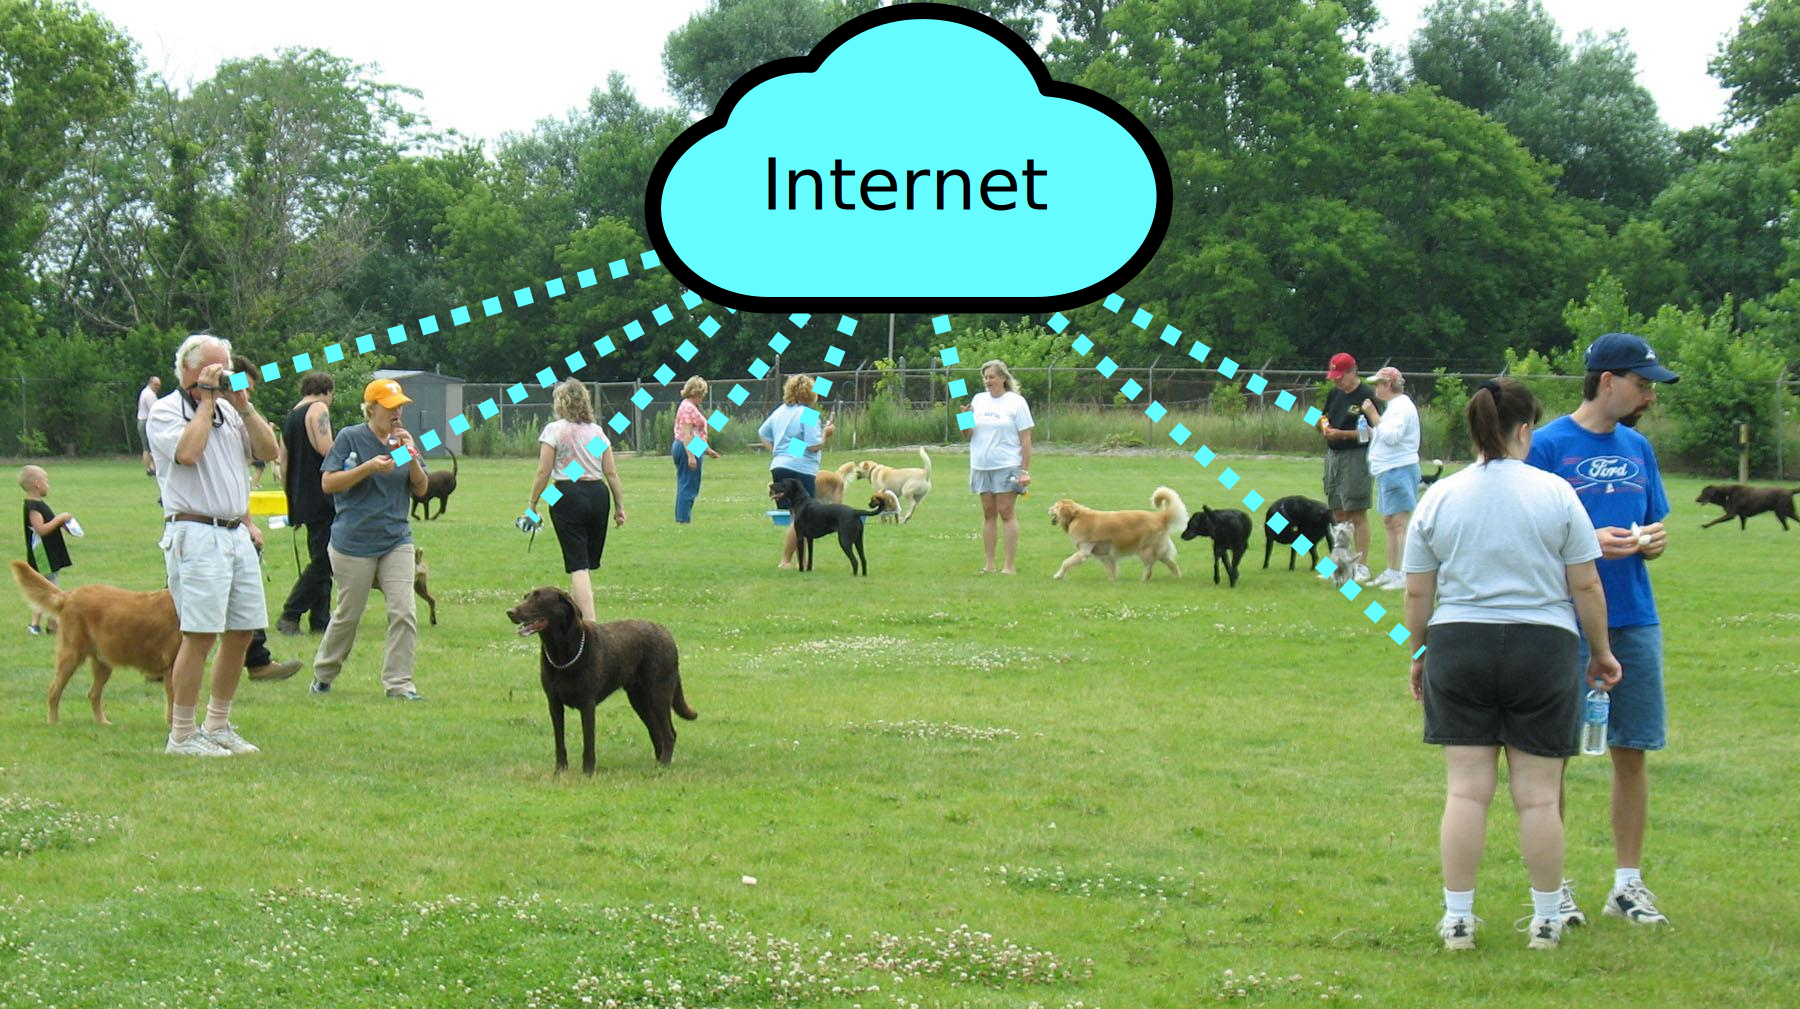
\includegraphics[width=0.99\textwidth]{imgs/random_people} 
  \end{figure}
\end{frame}

\begin{frame}{Big crowds}
  \centering
  \scriptsize
  \begin{figure}
    \includegraphics[width=0.90\textwidth]{imgs/rome_marathon} 
  \end{figure}
\end{frame}

\begin{frame}{Big crowds and cloud don't play well}
  \centering
  \scriptsize
  \begin{figure}
    \includegraphics[width=0.90\textwidth]{imgs/no_internet} 
  \end{figure}
\end{frame}

\begin{frame}{Big crowds and cloud don't play well}
  \centering
  \scriptsize
  \begin{figure}
    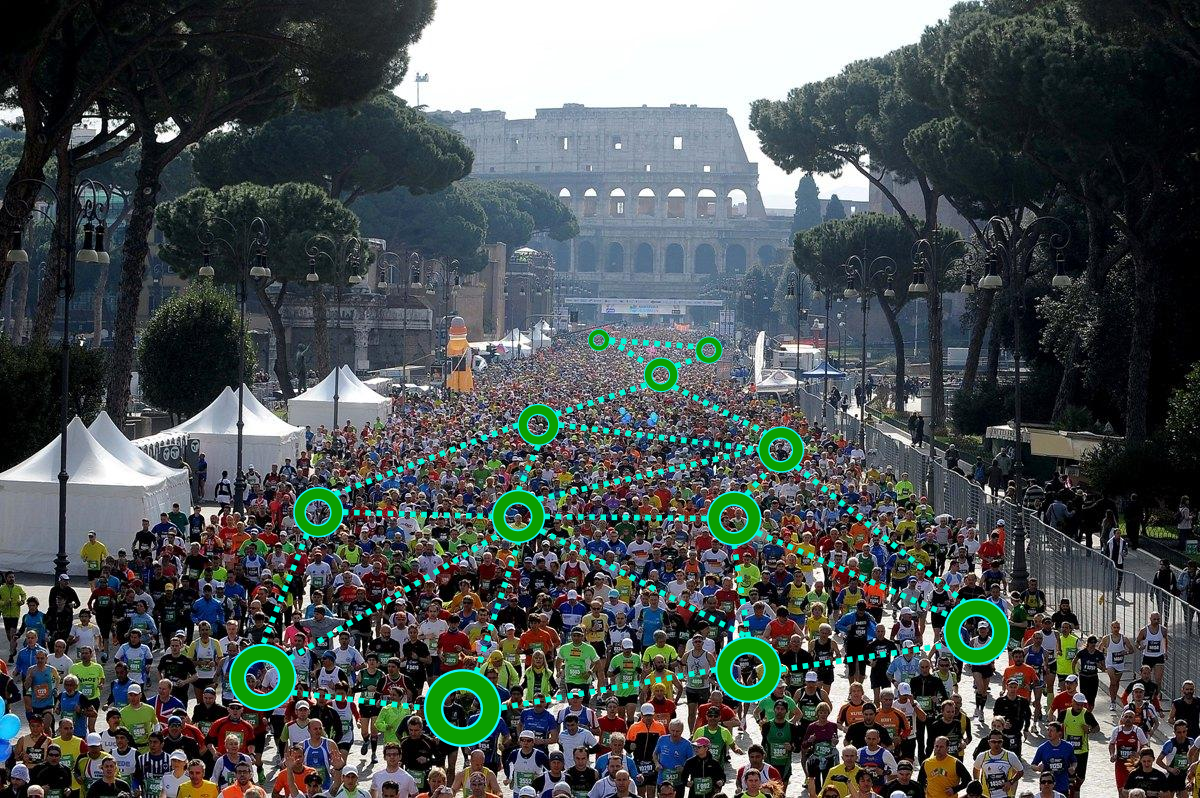
\includegraphics[width=0.90\textwidth]{imgs/rome_mesh} 
  \end{figure}
\end{frame}

\begin{frame}{Big crowds and dangers}
  \centering
  \scriptsize
  Photo: Sam Panthanky/AFP/Getty Images
  \begin{figure}
    \includegraphics[width=0.85\textwidth]{imgs/india_stampede} 
  \end{figure}
\end{frame}

\begin{frame}{Big crowds and dangers}
  \begin{block}{Crowd disasters}
    \begin{itemize}
     \item July 24, 2010 -- Germany, Duisburg -- 21 deaths
     \item January 1, 2013 -- Ivory Coast, Abidjan -- 60 deaths
     \item February 20, 2003 -- USA, Rhode Island -- 100 deaths
     \item October 13, 2013 -- India, Madhya Pradesh, Datia -- 115 deaths
     \item May 9, 2001 -- Ghana, Accra -- 126 deaths
     \item January 23, 2013 -- Brazil, Santa Maria -- 242 deaths
     \item January 12, 2006 -- Saudi Arabia, Mecca -- 345 deaths
     \item November 22, 2010 -- Cambodia, Phnom Penh -- 347 deaths
     \item August 31, 2005 -- Iraq, Baghdad -- 1000 deaths
     \item This is a small list of stampedes, there are thousands more.
    \end{itemize}
  \end{block}
\end{frame}



\begin{frame}{Channel}
  \centering
  \begin{figure}
    \includegraphics[width=0.6\textwidth]{imgs/channel-wide} 
  \end{figure}
\end{frame}

\begin{frame}\frametitle{Crowd sensitive steering benefits: data}
  \begin{figure}
  \includegraphics[width=0.99\textwidth]{imgs/chart}
  \end{figure}
  \Tiny{Number of users surrounding the user (within 100 meters from her).
  %
  With ``normalised distance'', we mean that we divided the distance the user still has to walk to reach the target by the total length of the suggested path.}
\end{frame}





\end{document}
